%!TEX root = ../paper.tex
%\begin{figure*}[h]
%     \subfloat[Throughput vs. Clock]{%
%       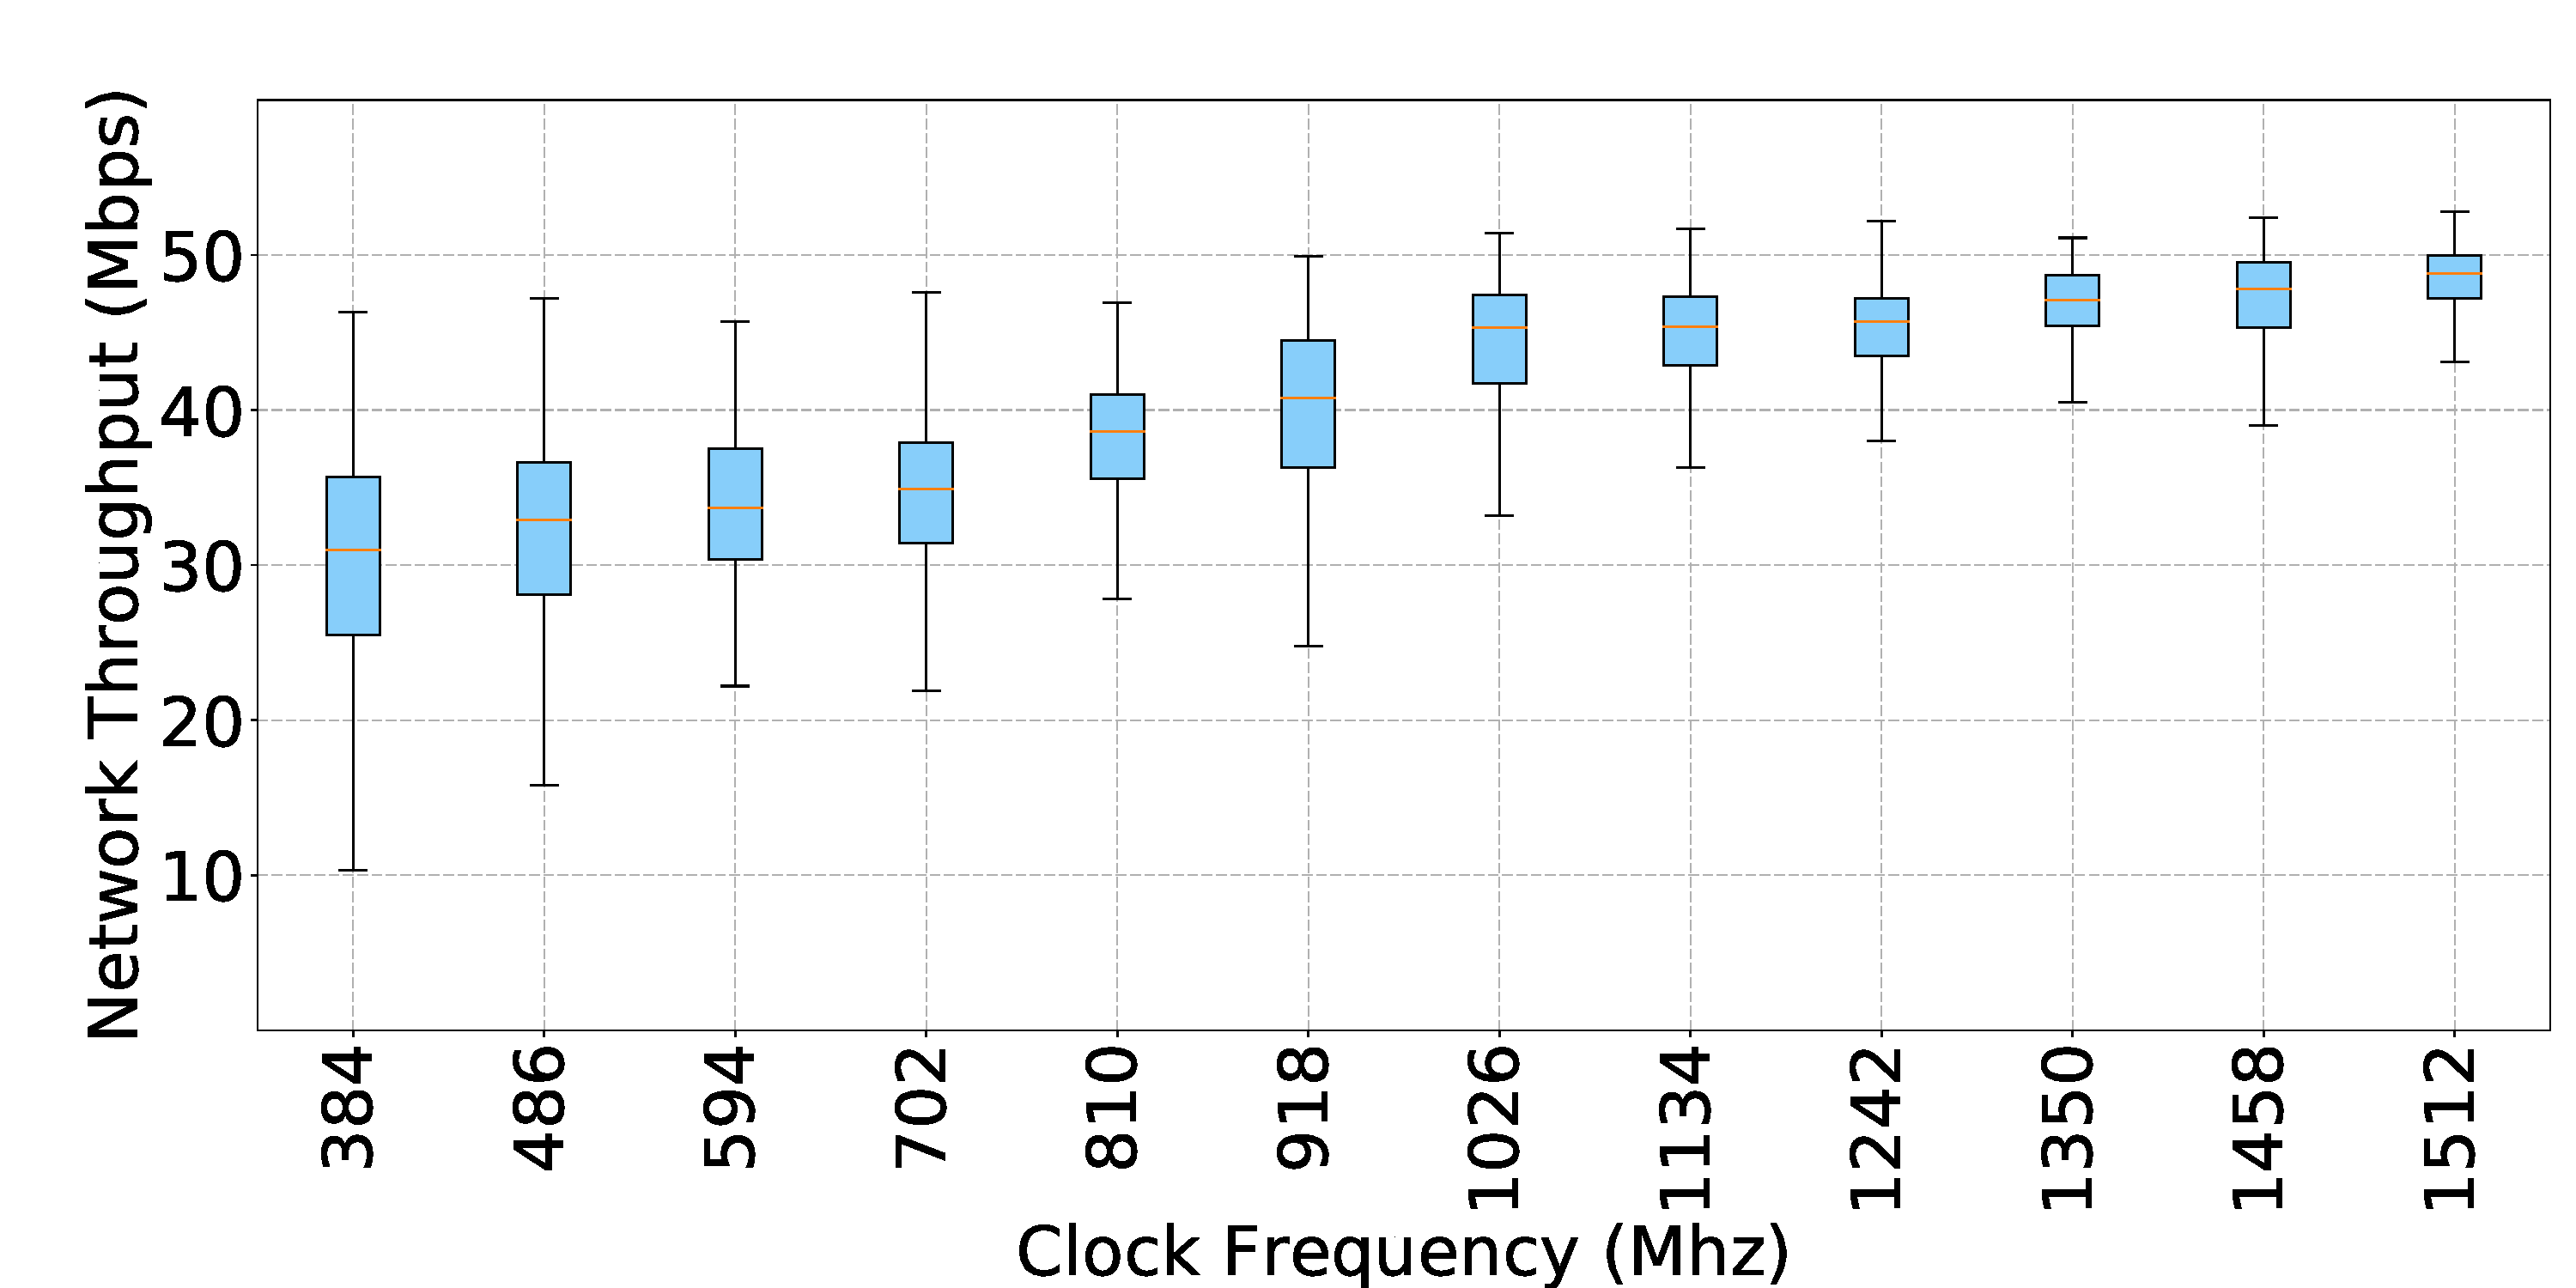
\includegraphics[height=0.27\textwidth,width=0.5\textwidth]{sections/Throughput}
%     }
%     \subfloat[Packet processing delay vs. Clock]{%
%       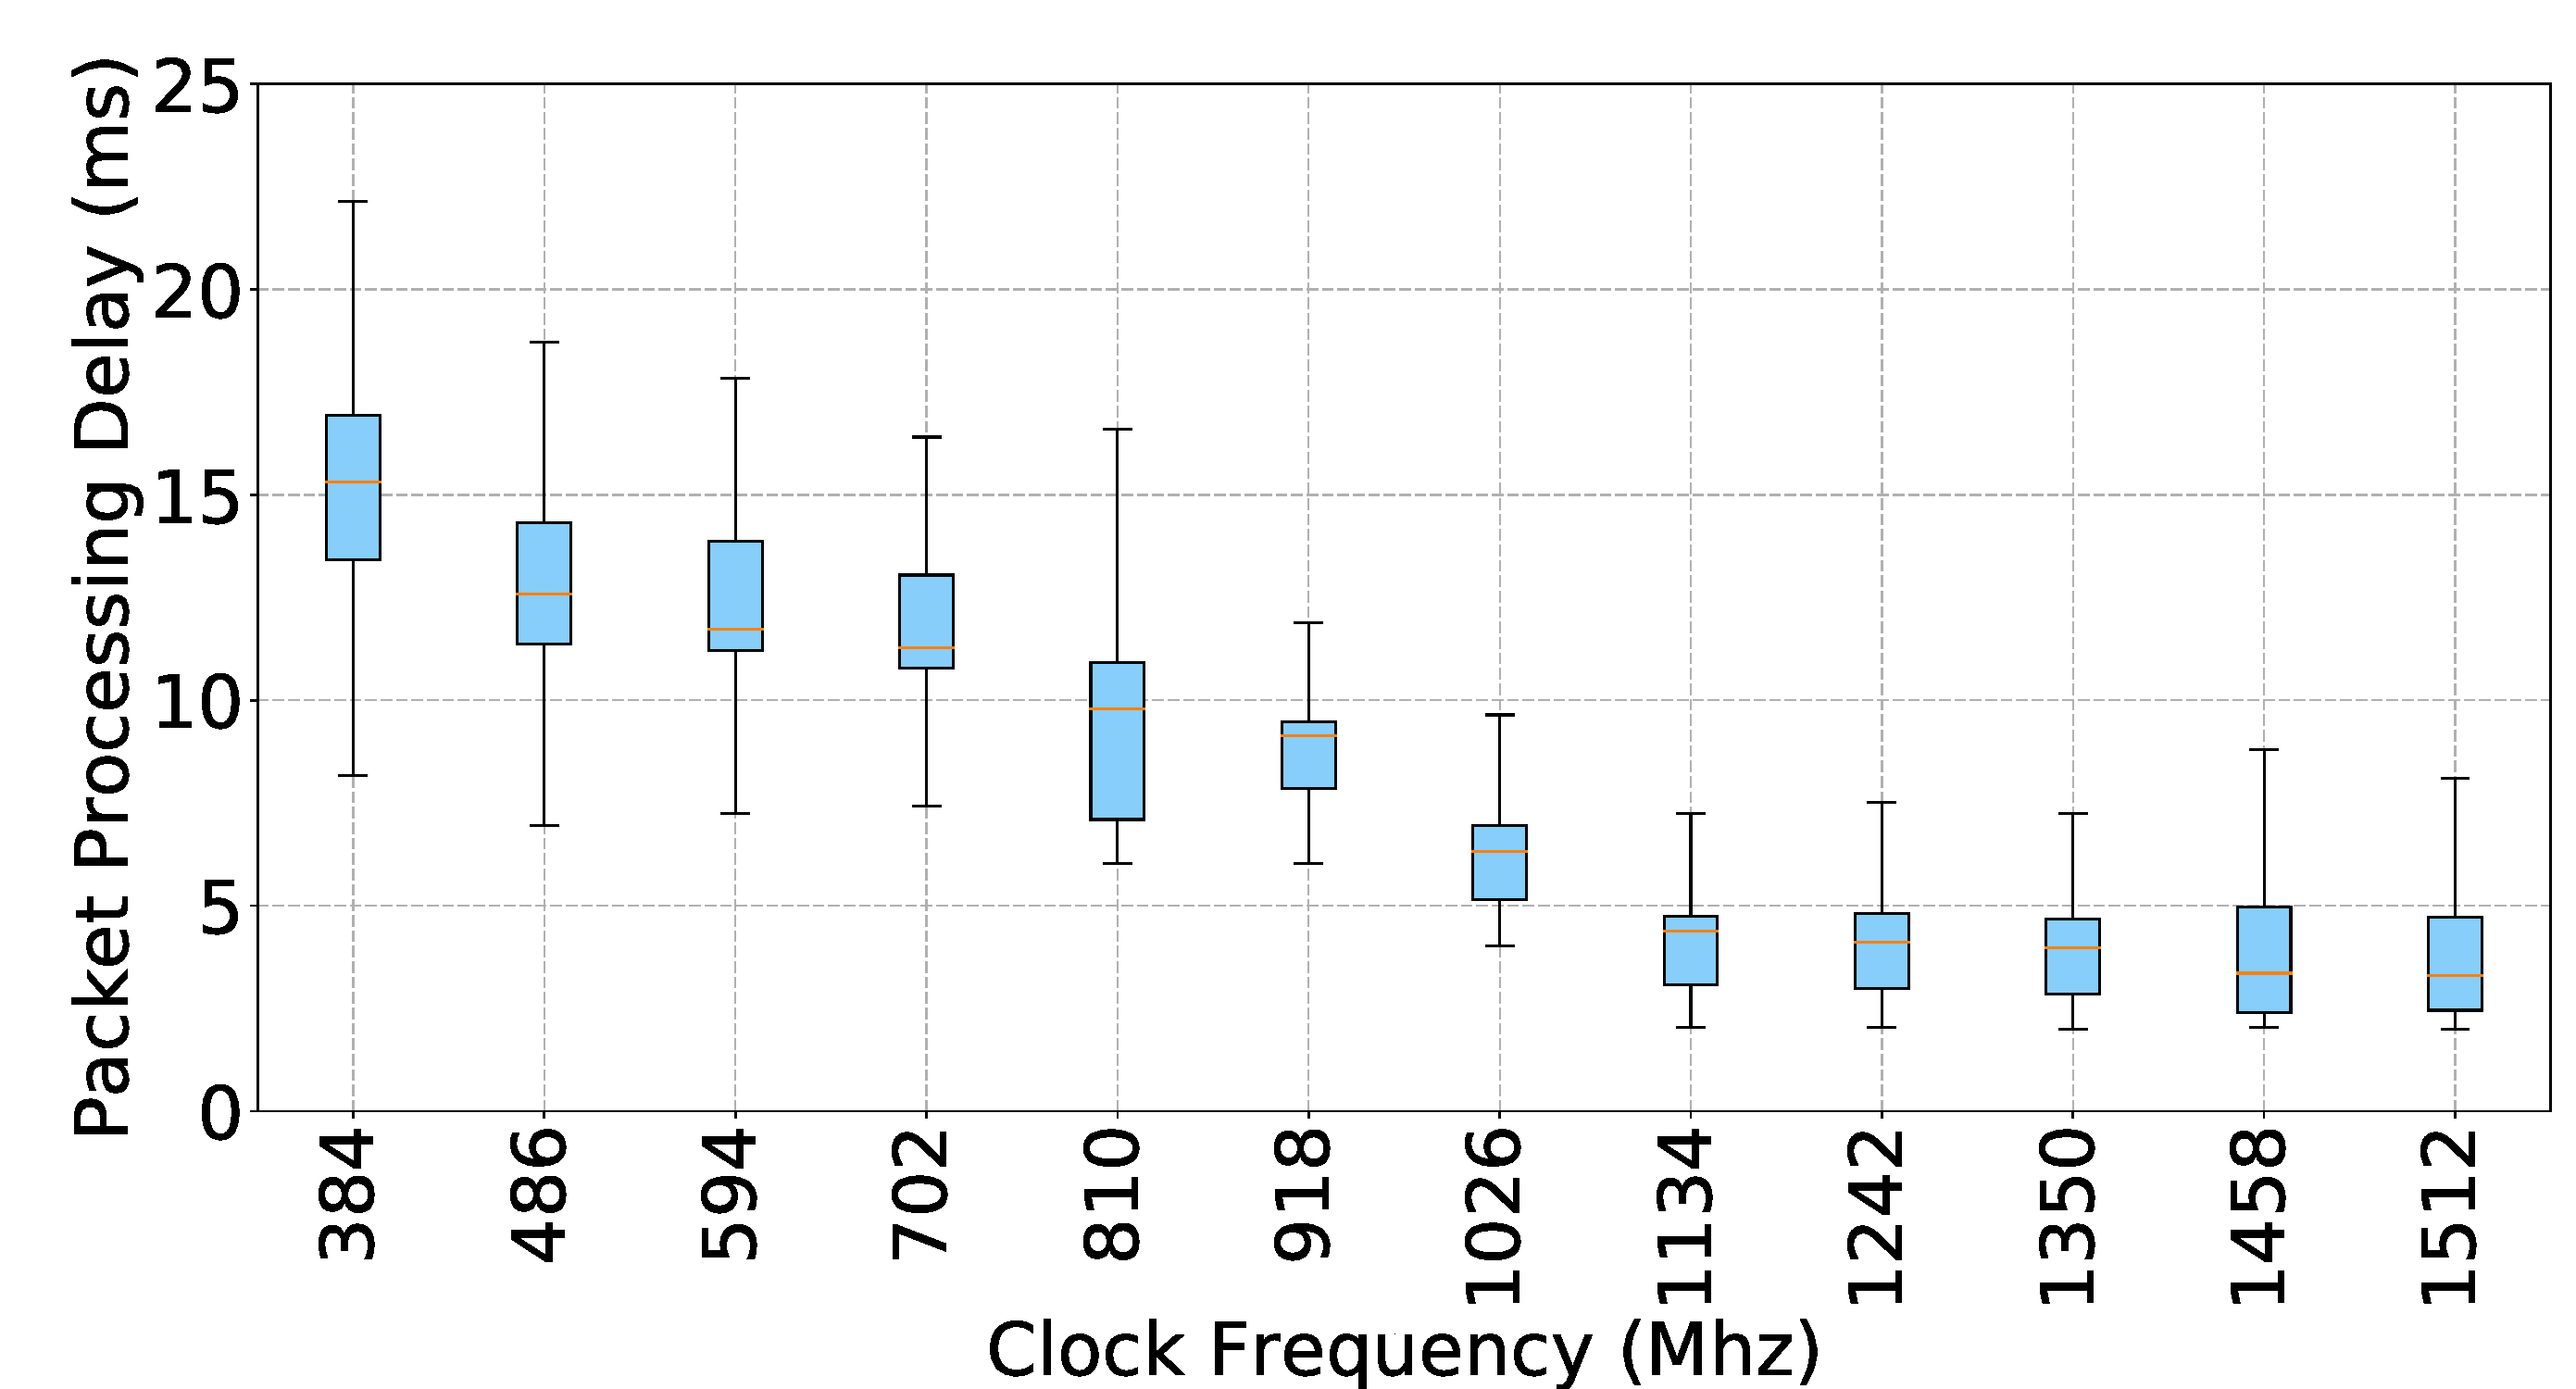
\includegraphics[height=0.27\textwidth,width=0.5\textwidth]{sections/ppd}
%     }
%     \vspace{-0.1in}
%     \caption{Second-order effect of CPU speed on network. (a) TCP throughput reduces from an average of 48 Mbps to 32 Mbps under slow clock under the same network conditions, b) The cause for this reduction in throughput is internal to the device; the average TCP packet processing delay increases by 12 ms at slow CPU speeds. Experiments conducted on Nexus 4.}
%     \label{fig:tcp-perf}
%\end{figure*}

\begin{figure*}[t]
  \centering
  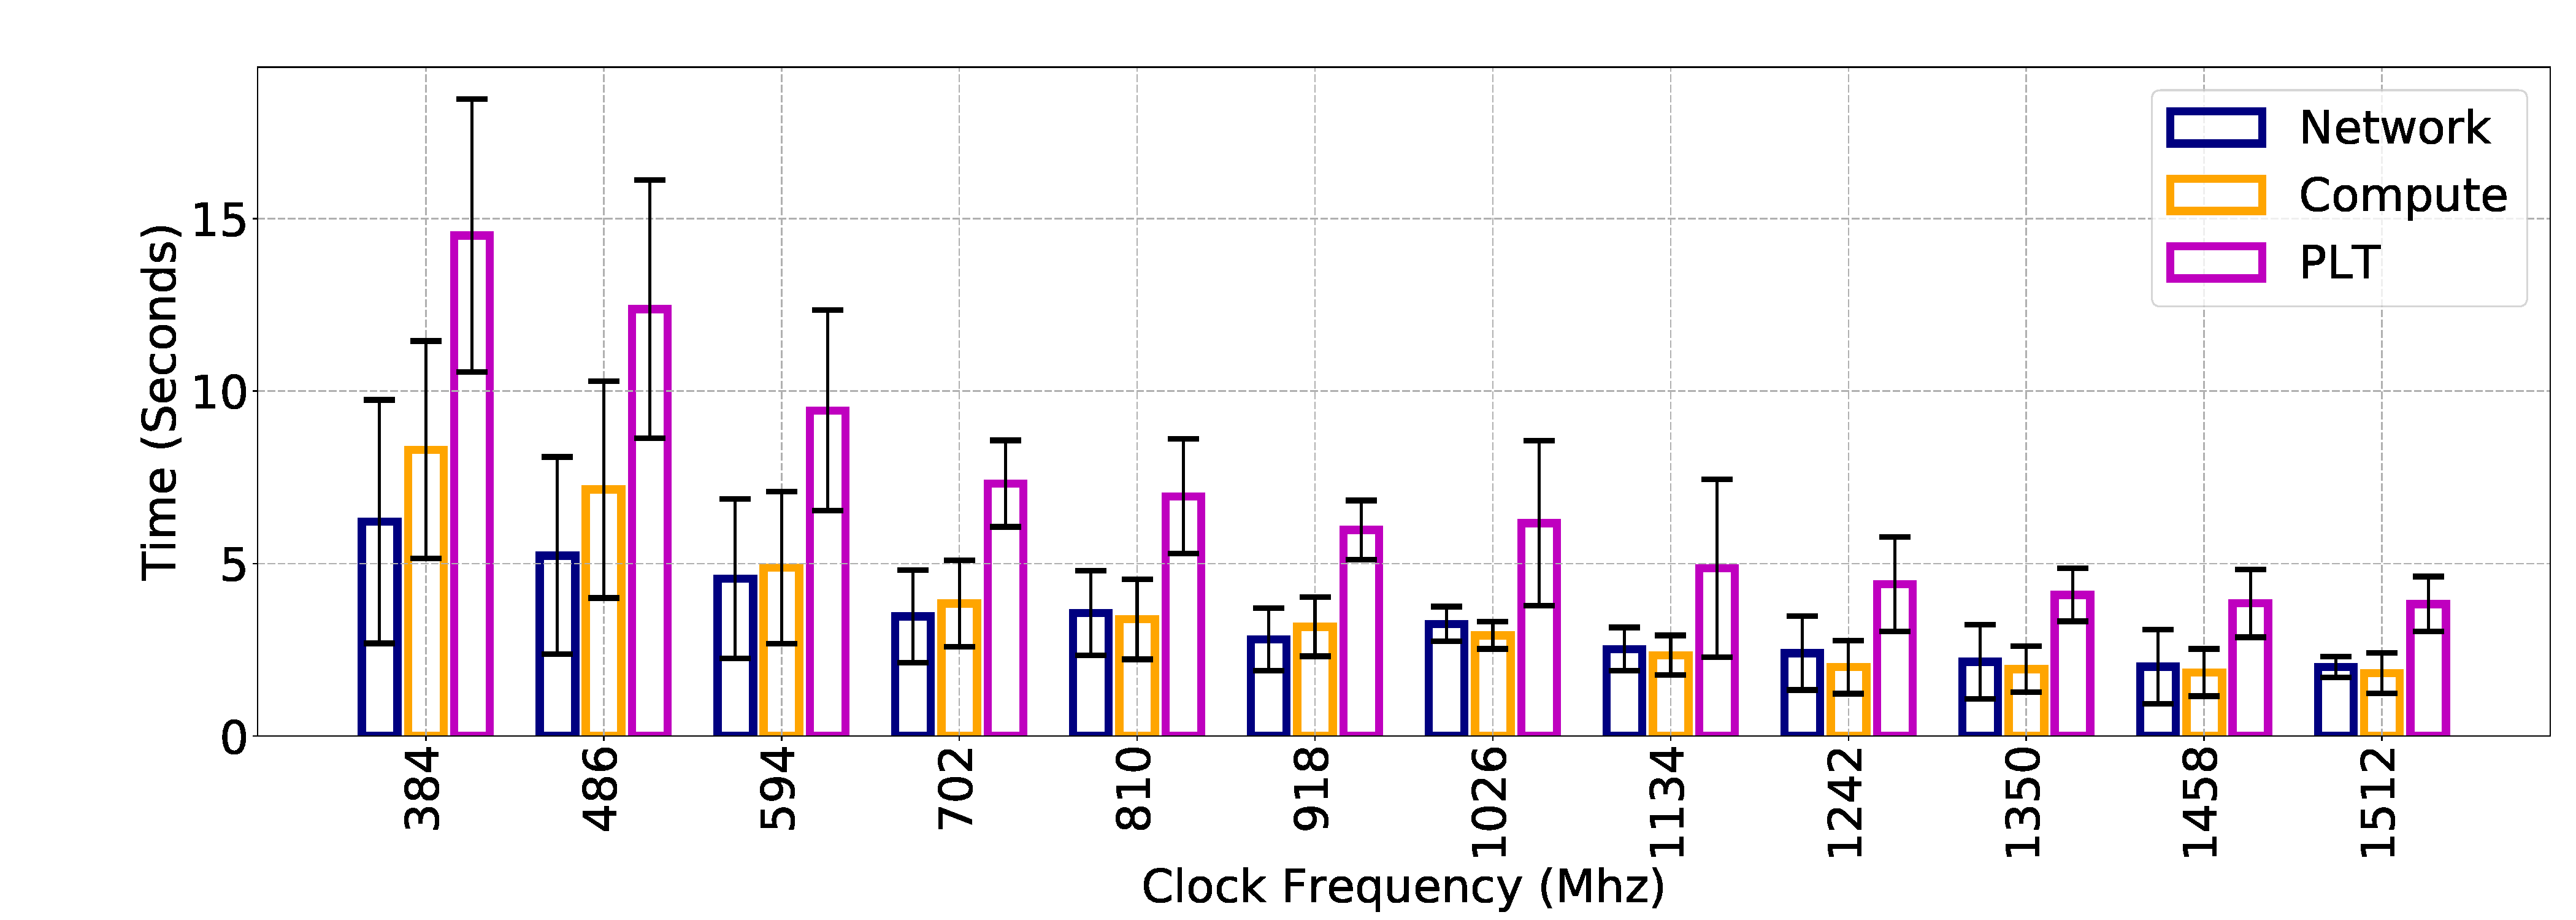
\includegraphics[width=0.8\linewidth]{sections/device-work/plt-isolate.pdf}
    \caption{Isolating the effect of network activities and compute activities as the CPU speed changes. The PLT of the Web page is the sum of the time taken for compute activities and the time taken for the network activities on the critical path~\cite{wang2013demystifying,nejati2016depth}. The PLT is the same as that shown in Figure~\ref{fig:plt_clock}. As the CPU slows down, the compute activities are affected more than the network activities. }\vspace{-0.2in}
  \label{fig:plt_isolate}
\end{figure*}

\begin{figure}[t]
  \centering
  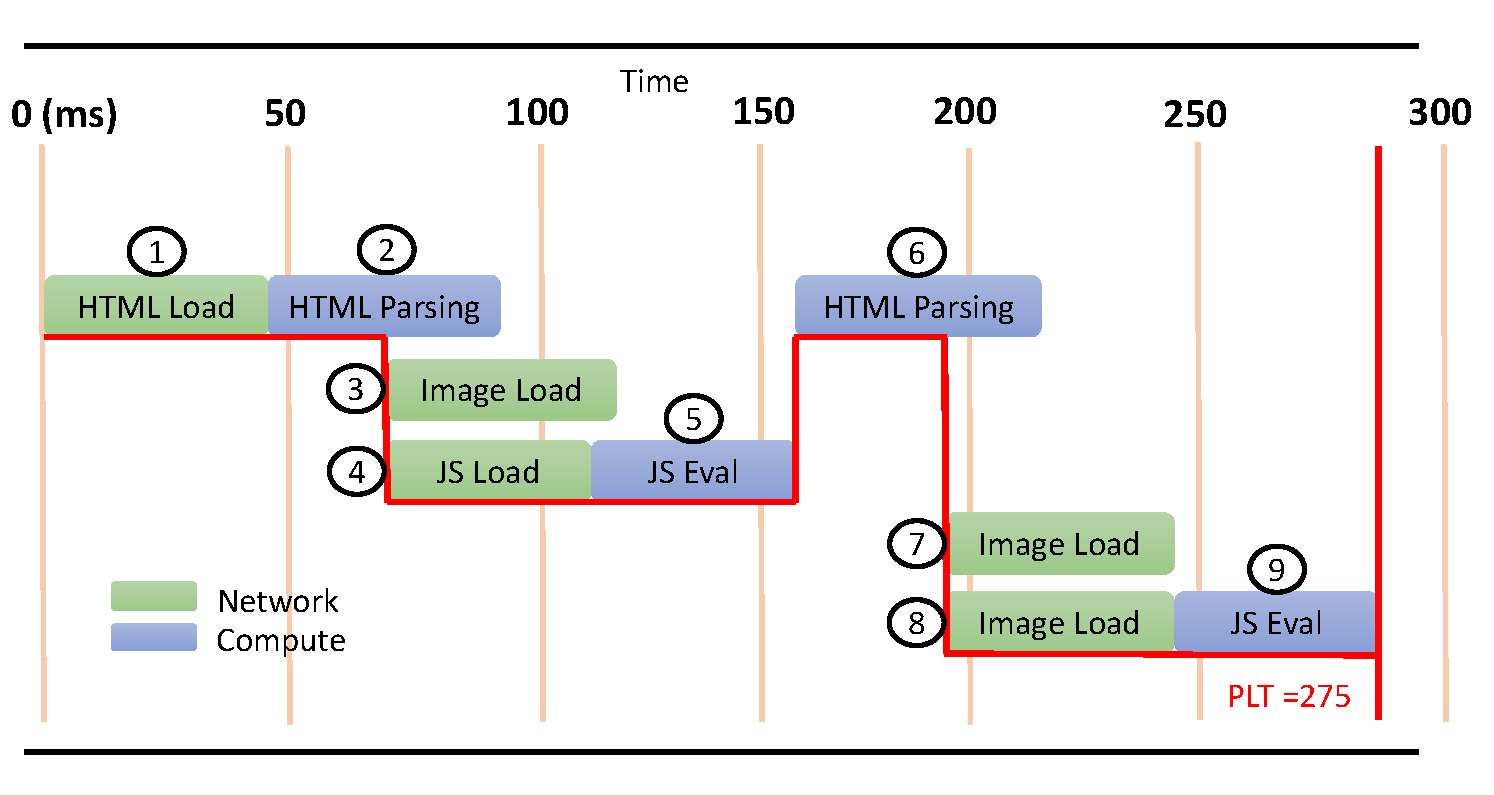
\includegraphics[width=\linewidth]{sections/device-work/wprof-dp.pdf}
    \caption{An example page load process divided into its network and compute activities, obtained from the WProf tool~\cite{wang2013demystifying,nejati2016depth}. The red line shows the critical path during the page load process, and represents the page load time. }
  \label{fig:wprof-dp}
\end{figure}

\subsection{Second-Order Effect of CPU Clock on the Network} \label{label:throughput}

One of our findings when studying the impact of CPU speed on application performance is that 
the CPU clock not only affects application processing, {\em but has a second-order effect on network 
latency/throughput because of the packet processing delays.} This in turn impacts
application performance as well. In our experiment, we generate traffic using the IPerf tool~\cite{iperf-2015} from a server to the Nexus 4 smartphone. IPerf generates continuous traffic, and we measure the average throughput over 5 minutes duration. We repeat the experiment 20 times for 12 different CPU clock frequencies. 
%to send continuous data from a server to the Nexus 4 smartphone \todo{how long is the experiment?}. We estimate the average throughput 

Fig. \ref{fig:tcp-perf}a shows the effect of clock on network throughput. When the clock frequency is reduced from 1512 MHz to 384 MHz, the average throughput drops from 48 Mbps to 32 Mbps. This decrease in throughput is entirely internal to the device. Recall (\S\ref{sec:setup}) that in our set up, the network condition is held near-constant since we use an over-provisioned LAN and the video and Web content are served from a server located in the LAN. 

The reason for the decreased TCP throughput is that packet processing is compute intensive, and a slow CPU increases the packet processing delays. Figure~\ref{fig:tcp-perf}b shows the average delay to process a packet under different clock frequencies for the same IPerf experiment. Android timestamps packets when it reaches the kernel which can be obtained using the IOCTL system call. We measure the packet processing delay as the time between when the packet reaches the application and when it is received at the kernel.

Figure~\ref{fig:tcp-perf}b shows that the packet processing delay when the CPU frequency is 384 MHz is 
12\,ms more compared to when the CPU frequency is 1512\,MHz, per packet. This increase in packet processing significantly affects TCP throughput, even when the network conditions remain the same. We repeated these experiments on the higher end Google Pixel 2 phone and found similar trends; even though the packet processing was considerably faster ($<$ 2ms under high clock) compared to Nexus 4, the difference in processing between the slow and the fast CPU frequency settings was 10ms.  

This second-order effect has significant implications.  The CPU capacity can affect application QoE both by slowing down the compute and the network components of the application. Isolating these effects is critical for designing new optimizations.

